\section{Fluxes}
\label{sec:fluxes}
%
In order to investigate the turbulent particle flux, we first note that the density flux in a single point tells us little about the particle flux out of the system.
Potentially a positive flux the specified point could be outbalanced by a negative outflux in another point.
We will therefore integrate the perpendicular density flux over a surface $\mathcal{S}$, which gives us the particle flux with units (particles) $s^{-1}$.
It would seem that letting $\mathcal{S}$ be the simulation domain would make sense.
However, as we have enforce $\phi=0$ at $\rho=L_\rho$, $u_{E,\rho}=0$ as $\partial_\theta \phi=0$ (see \cref{poi:cylExB}).
As a side note, we note that very little plasma cannot escape the simulation domain radially as $\phi=0$, and because the Neumann condition on the density at the outer radius gives a diffusion of $\partial_\rho^2 n \simeq 0$.
Hence almost all the plasma escapes in the parallel direction.

As we would like to investigate the radial turbulent particle flux, we therefore set the radius of $\mathcal{S}$ to be away from the region where $\phi=0$ enforcement starts, but still outside the main part of the particle source.
The result is shown in \cref{fig:flux0008}, and gives a comparison to the parallel density flux out of the simulation domain.
%
\begin{figure}[htb]
    \centering
    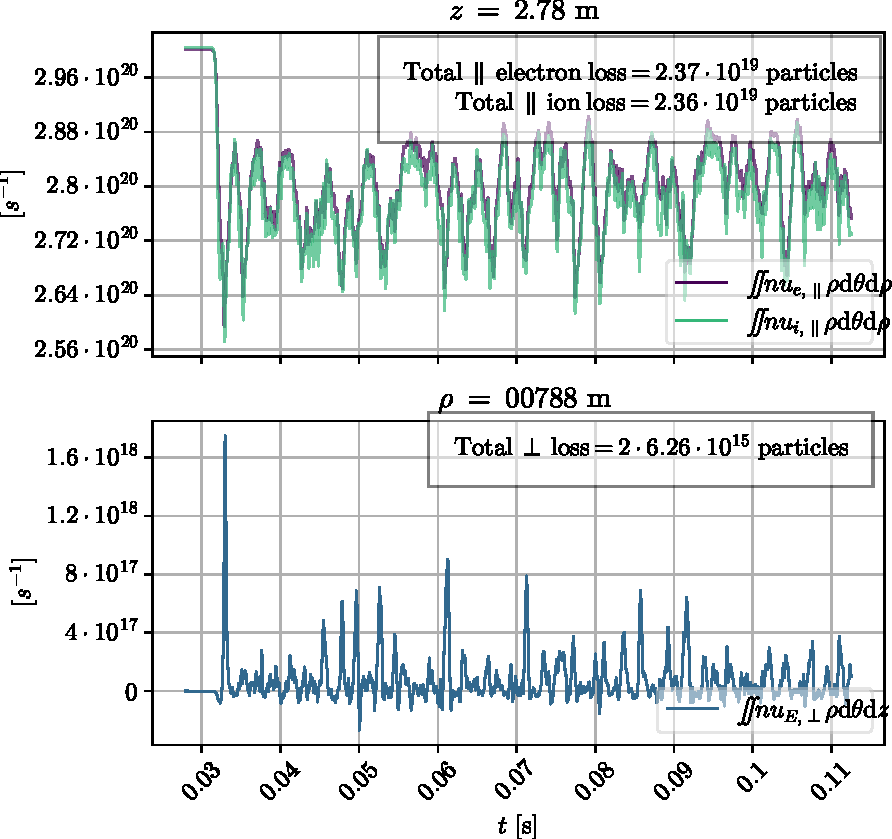
\includegraphics{fig/results/totalFlux/flux0008}
    \caption{Integrated flux for $B=0.08\T$}
    \label{fig:flux0008}
\end{figure}
%
In the linear phase after $0.02\s$, the radial flux is almost zero due to the small amplitudes of the fluctuations in potential and density.
An overshoot just like the one seen in \cref{fig:energyTrace008} follows the linear phase.
From that point in time the radial flux comes burstwise throughout the simulation.

Although the particles are not escaping the domain in the perpendicular direction, the total perpendicular particle flux (i.e. the particle flux integrated over time) through $\mathcal{S}$
is approximately $10\%$ of the parallel flux out of the domain.

Finally, we mention that we are not solving $u_{i,\|}$ and $u_{e,\|}$ in time, but rather $j_{\|}$ and $nu_{i,\|}$.
Dispite of this, we can see that there almost as many ions as electrons are lost in the parallel direction (up to $99\%$).
Physically, this means that the plasma is charging up very little over time, and the that quasi-neutrality holds.
